%%
%% This is a cleaned academic paper template based on ACM SIGPLAN format
%%
\documentclass[sigconf,authorversion,nonacm]{acmart}

\usepackage{booktabs}
\usepackage{graphicx}
\usepackage{subfigure}
\usepackage{algorithm}
\usepackage{algorithmicx}
\usepackage{algpseudocode}
\usepackage{tikz}
\usepackage{pgfplots}
\usepackage{xcolor}
\usepackage{float}
\usepackage{natbib}


%%
%% \BibTeX command to typeset BibTeX logo in the docs
\AtBeginDocument{%
  \providecommand\BibTeX{{%
    Bib\TeX}}}

%% Rights management information - UPDATE THESE VALUES
% \setcopyright{acmlicensed}
% \copyrightyear{2024}
% \acmYear{2024}
% \acmDOI{10.1145/3XXX.3XXX}

%% Conference information - UPDATE THESE VALUES
% \acmConference[ASPLOS '24]{29th ACM International Conference on Architectural Support for Programming Languages and Operating Systems}{April 27--May 1, 2024}{La Jolla, CA, USA}
% \acmISBN{978-1-4503-XXXX-X/2024/04}

%%
%% end of the preamble, start of the body of the document source.
\begin{document}

%%
%% The "title" command has an optional parameter for short title in headers
\title{LLM-Enhanced Memory Prefetching: Evaluating Gemini's Capability for Program Counter and Delta Prediction}

%%
%% Author information - UPDATE WITH YOUR DETAILS
\author{Jayden Lin}
\email{jaydenl@andrew.cmu.edu}
\orcid{0000-0000-0000-0000}
\affiliation{%
  % \institution{UBC}
  % \streetaddress{123 University Ave}
  % \city{Your City}
  % \state{Your State}
  % \postcode{12345}
  % \country{USA}
}

% \author{Co-Author Name}
% \email{coauthor@institution.edu}
% \affiliation{%
%   \institution{Your Institution}
%   \streetaddress{123 University Ave}
%   \city{Your City}
%   \state{Your State}
%   \postcode{12345}
%   \country{USA}
% }

%%
%% For multiple authors, define short author list for headers
% \renewcommand{\shortauthors}{Your Name et al.}

%%
%% The abstract
% \begin{abstract}
% \textbf{Fairy Tale Abstract:} Once upon a time, computer systems relied on simple hardware prefetchers that could only detect basic sequential and strided memory access patterns, leaving complex, irregular program behaviors unpredictable and causing processors to waste precious cycles waiting for data to arrive from slow memory. But there lurked a terrible villain called Cache Misses, who delighted in forcing processors to stall and wait hundreds of cycles whenever programs accessed memory addresses that couldn't be predicted by traditional prefetching schemes, especially when applications exhibited intricate delta patterns and non-linear memory traversals that confounded conventional hardware predictors. Then emerged a mighty hero named Gemini, a large language model trained to recognize complex patterns in program counter sequences and their associated memory address deltas, wielding the power to predict future memory accesses by learning from historical execution traces and understanding the subtle relationships between program flow and data locality. With Gemini's pattern recognition abilities, processors could finally prefetch the right data at the right time, dramatically reducing cache misses and execution stalls, allowing programs to run faster and more efficiently, and thus programmers and computer users lived happily ever after with their lightning-fast applications.
% \end{abstract}
\begin{abstract}
Memory prefetching remains a bottleneck in modern computer systems, where traditional hardware prefetchers struggle with irregular access patterns characteristic of increasingly complex applications. While sequential and stride-based prefetchers effectively handle simpler memory patterns, they fail to predict certain nonlinear memory traversals, increasing latency from one to four cycles for a cache hit to tens to hundreds of cycles \cite{wilton2002cacti}, which translates to an exorbitant speed reduction. A prefetcher aims to load data intended for future use before it is requested, so the problem revolves around predicted where the useful data lie.

This paper incorporates Gemini, a large language model-based prefetching system that leverages transformer architectures to predict memory access patterns from program execution traces. Unlike conventional approaches that rely on fixed algorithmic patterns, Gemini attempts to learn relationships between program counter sequences and memory address deltas by training on historical execution data. This system attempts to capture dependencies and context-sensitive behaviors that traditional prefetchers do not have access to, in hopes of accurate prediction of memory address accesses.

% We evaluated Gemini across various datasets, hyperparameter settings, and prompt stylizations. Experimental results demonstrate substantial performance improvements, with cache miss reductions in optimal settings of X\% and overall execution time improvements of Y\% compared to state-of-the-art hardware prefetchers. 

Our findings indicate that large language models have the capability to prefetch for certain types of program executions, and may have the capacity to be trained for more nuanced ones. However, they are far too slow and inconsistent in their current states to be viable. With further developments, there may avenues that adapt to evolving software complexity. 
\end{abstract}

%%
%% CCS concepts - Generate these at https://dl.acm.org/ccs/ccs.cfm
% \begin{CCSXML}
% <ccs2012>
%  <concept>
%   <concept_id>10003120.10003138.10003139</concept_id>
%   <concept_desc>Human-centered computing~Ubiquitous and mobile computing</concept_desc>
%   <concept_significance>500</concept_significance>
%  </concept>
%  <concept>
%   <concept_id>10010520.10010553.10010562</concept_id>
%   <concept_desc>Computer systems organization~Embedded systems</concept_desc>
%   <concept_significance>300</concept_significance>
%  </concept>
% </ccs2012>
% </CCSXML}

% \ccsdesc[500]{Computer systems organization~Memory management}
% \ccsdesc[300]{Computing methodologies~Machine learning algorithms}
% \ccsdesc[100]{Software and its engineering~Software performance}

%%
%% Keywords - UPDATE WITH YOUR KEYWORDS
% \keywords{memory prefetching, large language models, program counter prediction, cache optimization, Gemini API, machine learning systems}

%%
%% Build the document header
\maketitle

\section{Introduction}
\label{sec:introduction}

Recent advances in large language models (LLMs) have demonstrated remarkable pattern recognition capabilities across diverse domains\cite{harte2023leveraging}. This paper explores the application of Google's Gemini model to the domain of memory prefetching, specifically investigating its ability to predict future memory access deltas based on program counter traces and historical access patterns.

Through systematic evaluation using program traces, we demonstrate that LLM-based prefetching can achieve impressive results for specific applications.


\section{Background and Motivation} \label{sec:background}

\subsection{The Memory Wall Problem}
Moore's law, though not perfectly accurate, states that the number of transistors in a chip doubles every two years. Processor performance has kept with this rapid growth, but memory access latency remains stagnant, fostering an ever-increasing disparity. Processors executing billions of operations per second must wait hundreds of cycles for data from main memory to proceed.

% Cache misses exemplify this bottleneck's severity, reducing performance by 10--50\% in memory-intensive applications including:
% \begin{itemize}
%     \item Database management systems
%     \item Scientific computing workloads  
%     \item Machine learning applications
% \end{itemize}

Memory prefetching offers a solution by loading data into faster cache levels before explicit processor requests. Successful prefetching transforms costly memory stalls into productive computation time, eliminating higher cache accesses that can take upwards of 20 times longer to complete \cite{wilton2002cacti}.

\subsection{Limitations of Current Prefetching}
Traditional hardware prefetchers detect patterns in simple access sequences but struggle with modern application complexity. Traditional approaches include \cite{mittal2016survey}:

\textbf{Sequential prefetchers:} Detect consecutive accesses and fetch subsequent cache lines

\textbf{Stride prefetchers:} Identify regular intervals and predict addresses using constant offsets  

\textbf{Stream buffers:} Record values from multiple concurrent access streams

\textbf{TAGE prefetchers:} Maintain limited historical context using tagged geometric history\\

These pattern-based methods perform worse on irregular access patterns increasingly common in modern software \cite{lee2012prefetching}. Applications featuring pointer-chasing, sparse matrices, tree traversals, and hash lookups exhibit complex, context-dependent behaviors that defy simple prediction. 

\subsection{Machine Learning's Advantages}

The sequential nature of program execution traces aligns naturally with transformer architectures designed for sequential modeling. Key advantages include:
\begin{itemize}
    \item Capturing long-range dependencies in memory access patterns
    \item Learning non-linear relationships between program context and memory behavior
    \item Adapting through fine-tuning for specific applications or domains
\end{itemize}

LLM-based prefetching could unlock significant performance gains for irregular workloads, while future work on fine tuning could allow programs to have individualized models, rather than a one-size-fits-all prefetching system. This approach provides program designers with significantly improved flexibility in data locality, highlighting machine learning's primary advantage in system design.

\subsection{Google Gemini's API}
Gemini API is free for the public use, which is why we have selected it for the trials in this paper. Other LLMs such as Claude, ChatGPT, DeepSeek, etc. either do not have an public API or are not applicable for research purposes. 


\newpage
\section{Methodology and Experimental Design}
\label{sec:design}

This study was conducted using seven pairs of benchmark traces, each simulating a distinct program execution. Each trace consists of program counters (PC) and the associated memory address deltas ($\Delta$), which are the differences between consecutive memory accesses. We systematically gather a number of consecutive PC-$\Delta$ pairs as a batch, then format it to fit into a question template that the Gemini API can respond to. In the request, Gemini is tasked to predict the subsequent $\Delta$ values without providing preamble or postamble. This response is defensively parsed to account for rare instances of unexpected tokens. These parsed $\Delta$ values are converted into a set of relative addresses where we can analyze them against the ground truth set.

There are many hyperparameters that can be varied during this process, which enables three types of experiments to determine optimal conditions for LLM prefetching:

\begin{enumerate}
    \item \textbf{Hyperparameter sweeps:} Given a specific dataset and prompt style, systematically test a matrix of input batch size and prediction lookahead size. For example, batch size can vary from 100--200 lines, while lookahead size can range from 30--80 lines.
    
    \item \textbf{Prompt comparison:} Given a specific parameter setting and dataset, make API calls with different prompts, ranging from minimal context to full explanations of the required task.
    
    \item \textbf{Dataset comparison:} Given a specific parameter setting and prompt style, test multiple datasets to determine which programs Gemini performs better on.
\end{enumerate}

We calculate four metrics: accuracy, precision, recall, and prediction duration. Each address prediction is treated as a binary true/false value through set intersection with the subsequent ground truth $\Delta$. Each configuration of hyperparameters undergoes 10 batch predictions to balance statistical reliability with computational feasibility. The metrics are then averaged and visualized through heatmaps and bar charts to facilitate comparison between parameter combinations.
\subsection{Prediction Pipeline}

\textbf{Figure~\ref{fig:pipeline}} illustrates our LLM-enhanced prefetching pipeline. The system operates in two main phases: (1) training data preparation and prompt engineering, and (2) inference and prediction evaluation.


\begin{figure}[t]
\centering
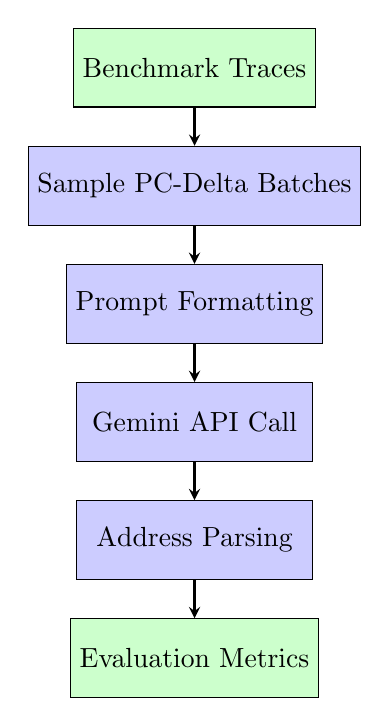
\begin{tikzpicture}[node distance=1.5cm, auto]
    % Define styles
    \tikzstyle{process} = [rectangle, minimum width=3cm, minimum height=1cm, text centered, draw=black, fill=blue!20]
    \tikzstyle{data} = [rectangle, minimum width=3cm, minimum height=1cm, text centered, draw=black, fill=green!20]
    \tikzstyle{arrow} = [thick,->,>=stealth]
    
    % Nodes in vertical arrangement
    \node [data] (traces) {Benchmark Traces};
    \node [process, below of=traces] (sample) {Sample PC-Delta Batches};
    \node [process, below of=sample] (prompt) {Prompt Formatting};
    \node [process, below of=prompt] (gemini) {Gemini API Call};
    \node [process, below of=gemini] (convert) {Address Parsing};
    \node [data, below of=convert] (evaluate) {Evaluation Metrics};
    
    % Arrows pointing down
    \draw [arrow] (traces) -- (sample);
    \draw [arrow] (sample) -- (prompt);
    \draw [arrow] (prompt) -- (gemini);
    \draw [arrow] (gemini) -- (convert);
    \draw [arrow] (convert) -- (evaluate);
\end{tikzpicture}
\caption{LLM Memory Prefetching System Pipeline}
\label{fig:pipeline}
\end{figure}

\subsection{Dataset Characteristics}

Our evaluation utilizes 7 distinct datasets derived from program execution traces. In the 50-Cache versions, the cache allocated for storing memory is double the size of the 25-Cache Versions, which causes slight differences in trace sizes as seen in \textbf{Table 1}. 

\begin{table}[h]
\centering
\caption{Dataset Characteristics}
\label{tab:datasets}
\begin{tabular}{@{}lrrr@{}}
\toprule
Dataset & 25-Cache Lines & 50-Cache Lines & Program Use\\
\midrule
cactu & 6.6 M & 2.2 M & ??\\
lrange & 121 M & 127 M & ??\\
mcf & 13.1 M & 1.3 M & ??\\
numpy & 17.6 M & 884 K & ??\\
omnetpp & 154 M & 62.4 M & ?? \\
pr & 393 M & 388 M & ??\\
ycsb-c & 42.3 M & 22.7 M & ??\\
\bottomrule
\end{tabular}
\end{table}

Each line contains a program counter and a memory access delta, representing the difference between consecutive memory address accesses.

\subsection{Experimental Configuration}

Table~\ref{tab:test-matrix} presents our main adjustable hyperparameters. 
% A setting is chosen in each of the columns to construct each trial, allowing for a very large number of possible experiments.

\begin{table*}[t]
\centering
\caption{Experimental Test Configuration Hyperparameters}
\label{tab:test-matrix}
% \medium
\begin{tabular}{@{}lrrrrrr@{}}
\toprule
Dataset & Input Batch Size & Prediction Size & Cache Size & Gemini Version & Prompt Style & Tuned\\
\midrule
cactu & 100 & 10 & 25 & 2.0 & Original & Yes\\
lrange & 125 & 20 & 50 & 2.5 & Minimal & No\\
mcf & 150 & 30 &  & & Contextual & \\
numpy & 175 & 40 &  & & Expert & \\
omnetpp & 200 & 50 &  &  &  & \\
pr & & 80 &  &  &  & \\
ycsb-c & & 70 & & &  &  \\

\bottomrule
\end{tabular}
\end{table*}

\subsection{Prompt Engineering Strategies}

We developed four distinct prompt engineering approaches:
\begin{enumerate}
    \item \textbf{Original}: The prompt explains that PC and delta pairs are given sequentially.
    \item \textbf{Minimal}: No context is given, just values. The prompt solely states to predict the next values in the sequence, with no differentiation between PC and delta.
    \item \textbf{Contextual}: The prompt opens with describing the context: "You are analyzing memory access patterns from a computer program" and also explains the meaning of PC and deltas. 
    \item \textbf{Expert}: The prompt gives Gemini a role and emphasizes the importance of accuracy: "You are an expert specializing in memory prefetching optimization. Your predictions are critical for system performance". Context is given as well.
\end{enumerate}



\begin{algorithm}[H]
\caption{Original Prompt Algorithm}
\label{alg:direct-prompt}
\begin{algorithmic}[1]
\State \textbf{Input:} Historical PC-Delta pairs $(pc_1, \Delta_1), ..., (pc_n, \Delta_n)$
\State \textbf{Template:} 
\State "Here are the most recent \{batch size\} program counter, delta pairs in sequential order (PC in hex, delta in decimal):"
\State "[PC-delta sequence]"
\State "Predict the next \{prediction size\} delta values with no other text or confirmations."
\State \textbf{Output:} Predicted deltas $\hat{\delta}_{n+1}, ..., \hat{\delta}_{n+N}$
\end{algorithmic}
\end{algorithm}

\section{Results and Discussion}
\label{sec:results-discussion}

\subsection{Model Version Comparison}

Figure~\ref{fig:model-comparison} compares the performance of Gemini 2.0 and 2.5 across metrics on the cactu dataset. Both models demonstrate similar performance in terms of accuracy, with hit rates of 89.7\% and 89.6\% respectively, precision scores of 90.6\% and 91.2\%, and recall values of 90.0\% and 90.2\%. The marginal differences in these core performance metrics are negligible.

However, a significant disparity emerges in inference time. Gemini 2.5 requires 25.2 seconds to complete 10 API calls, while Gemini 2.0 accomplishes the same task in only 3.7 seconds. Given that the performance improvements of Gemini 2.5 are minimal and do not justify the substantial increase in inference time, we selected Gemini 2.0 for all subsequent experiments.

\begin{figure}[h]
\centering
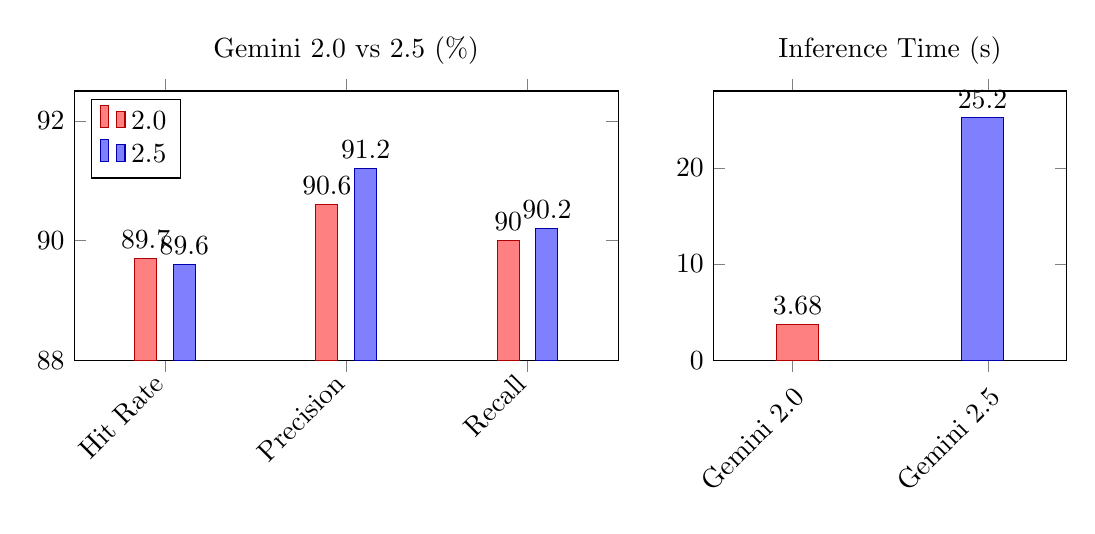
\begin{tikzpicture}
\begin{axis}[
    name=plot1,
    width=0.7\columnwidth,
    height=5cm,
    ymin=88, ymax=92.5,
    legend pos=north west,
    symbolic x coords={Hit Rate,Precision,Recall},
    xtick=data,
    x tick label style={anchor=east,rotate=45},
    ybar=0pt, % base bar separation
    bar width=8pt,
    enlarge x limits=0.25,
    title={Gemini 2.0 vs 2.5 (\%)},
    nodes near coords,
    nodes near coords align={vertical},
    every node near coord/.append style={text=black}
]


\addplot+[ybar, bar shift=-7pt, fill=red!50!white, draw=red!70!black] 
    coordinates {(Hit Rate,89.7) (Precision,90.6) (Recall,90.)};


\addplot+[ybar, bar shift=+7pt, fill=blue!50!white, draw=blue!70!black] 
    coordinates {(Hit Rate,89.6) (Precision,91.2) (Recall,90.20)};

\legend{2.0, 2.5}
\end{axis}



\begin{axis}[
    at={(plot1.south east)},
    anchor=south west,
    xshift=0.1\columnwidth,
    width=0.5\columnwidth,
    height=5cm,
    ylabel={},
    ymin=0, ymax=28,
    symbolic x coords={Gemini 2.0, Gemini 2.5},
    xtick={Gemini 2.0, Gemini 2.5},
    xticklabel style={rotate=45, anchor=north east},
    ybar=1.5pt,
    bar width=15pt,
    enlarge x limits=0.4,
    title={Inference Time (s)},
    % Add value labels on top of bars
    nodes near coords,
    nodes near coords align={vertical},
    every node near coord/.append style={text=black}
]
% Gemini 2.5 bar  

% Gemini 2.0 bar
\addplot+[ybar, bar shift=-2pt, fill=blue!50!white, draw=blue!70!black] coordinates {
    (Gemini 2.5,25.20)
};
\addplot+[ybar, bar shift=2pt, fill=red!50!white, draw=red!70!black]  coordinates {
    (Gemini 2.0,3.68)
};

\end{axis}


\end{tikzpicture}
\caption{Gemini models 2.0 and 2.5 performance comparison}
\label{fig:model-comparison}
\end{figure}

\subsection{Prompt Configuration Analysis}

% \begin{figure*}[t]
% \centering
% 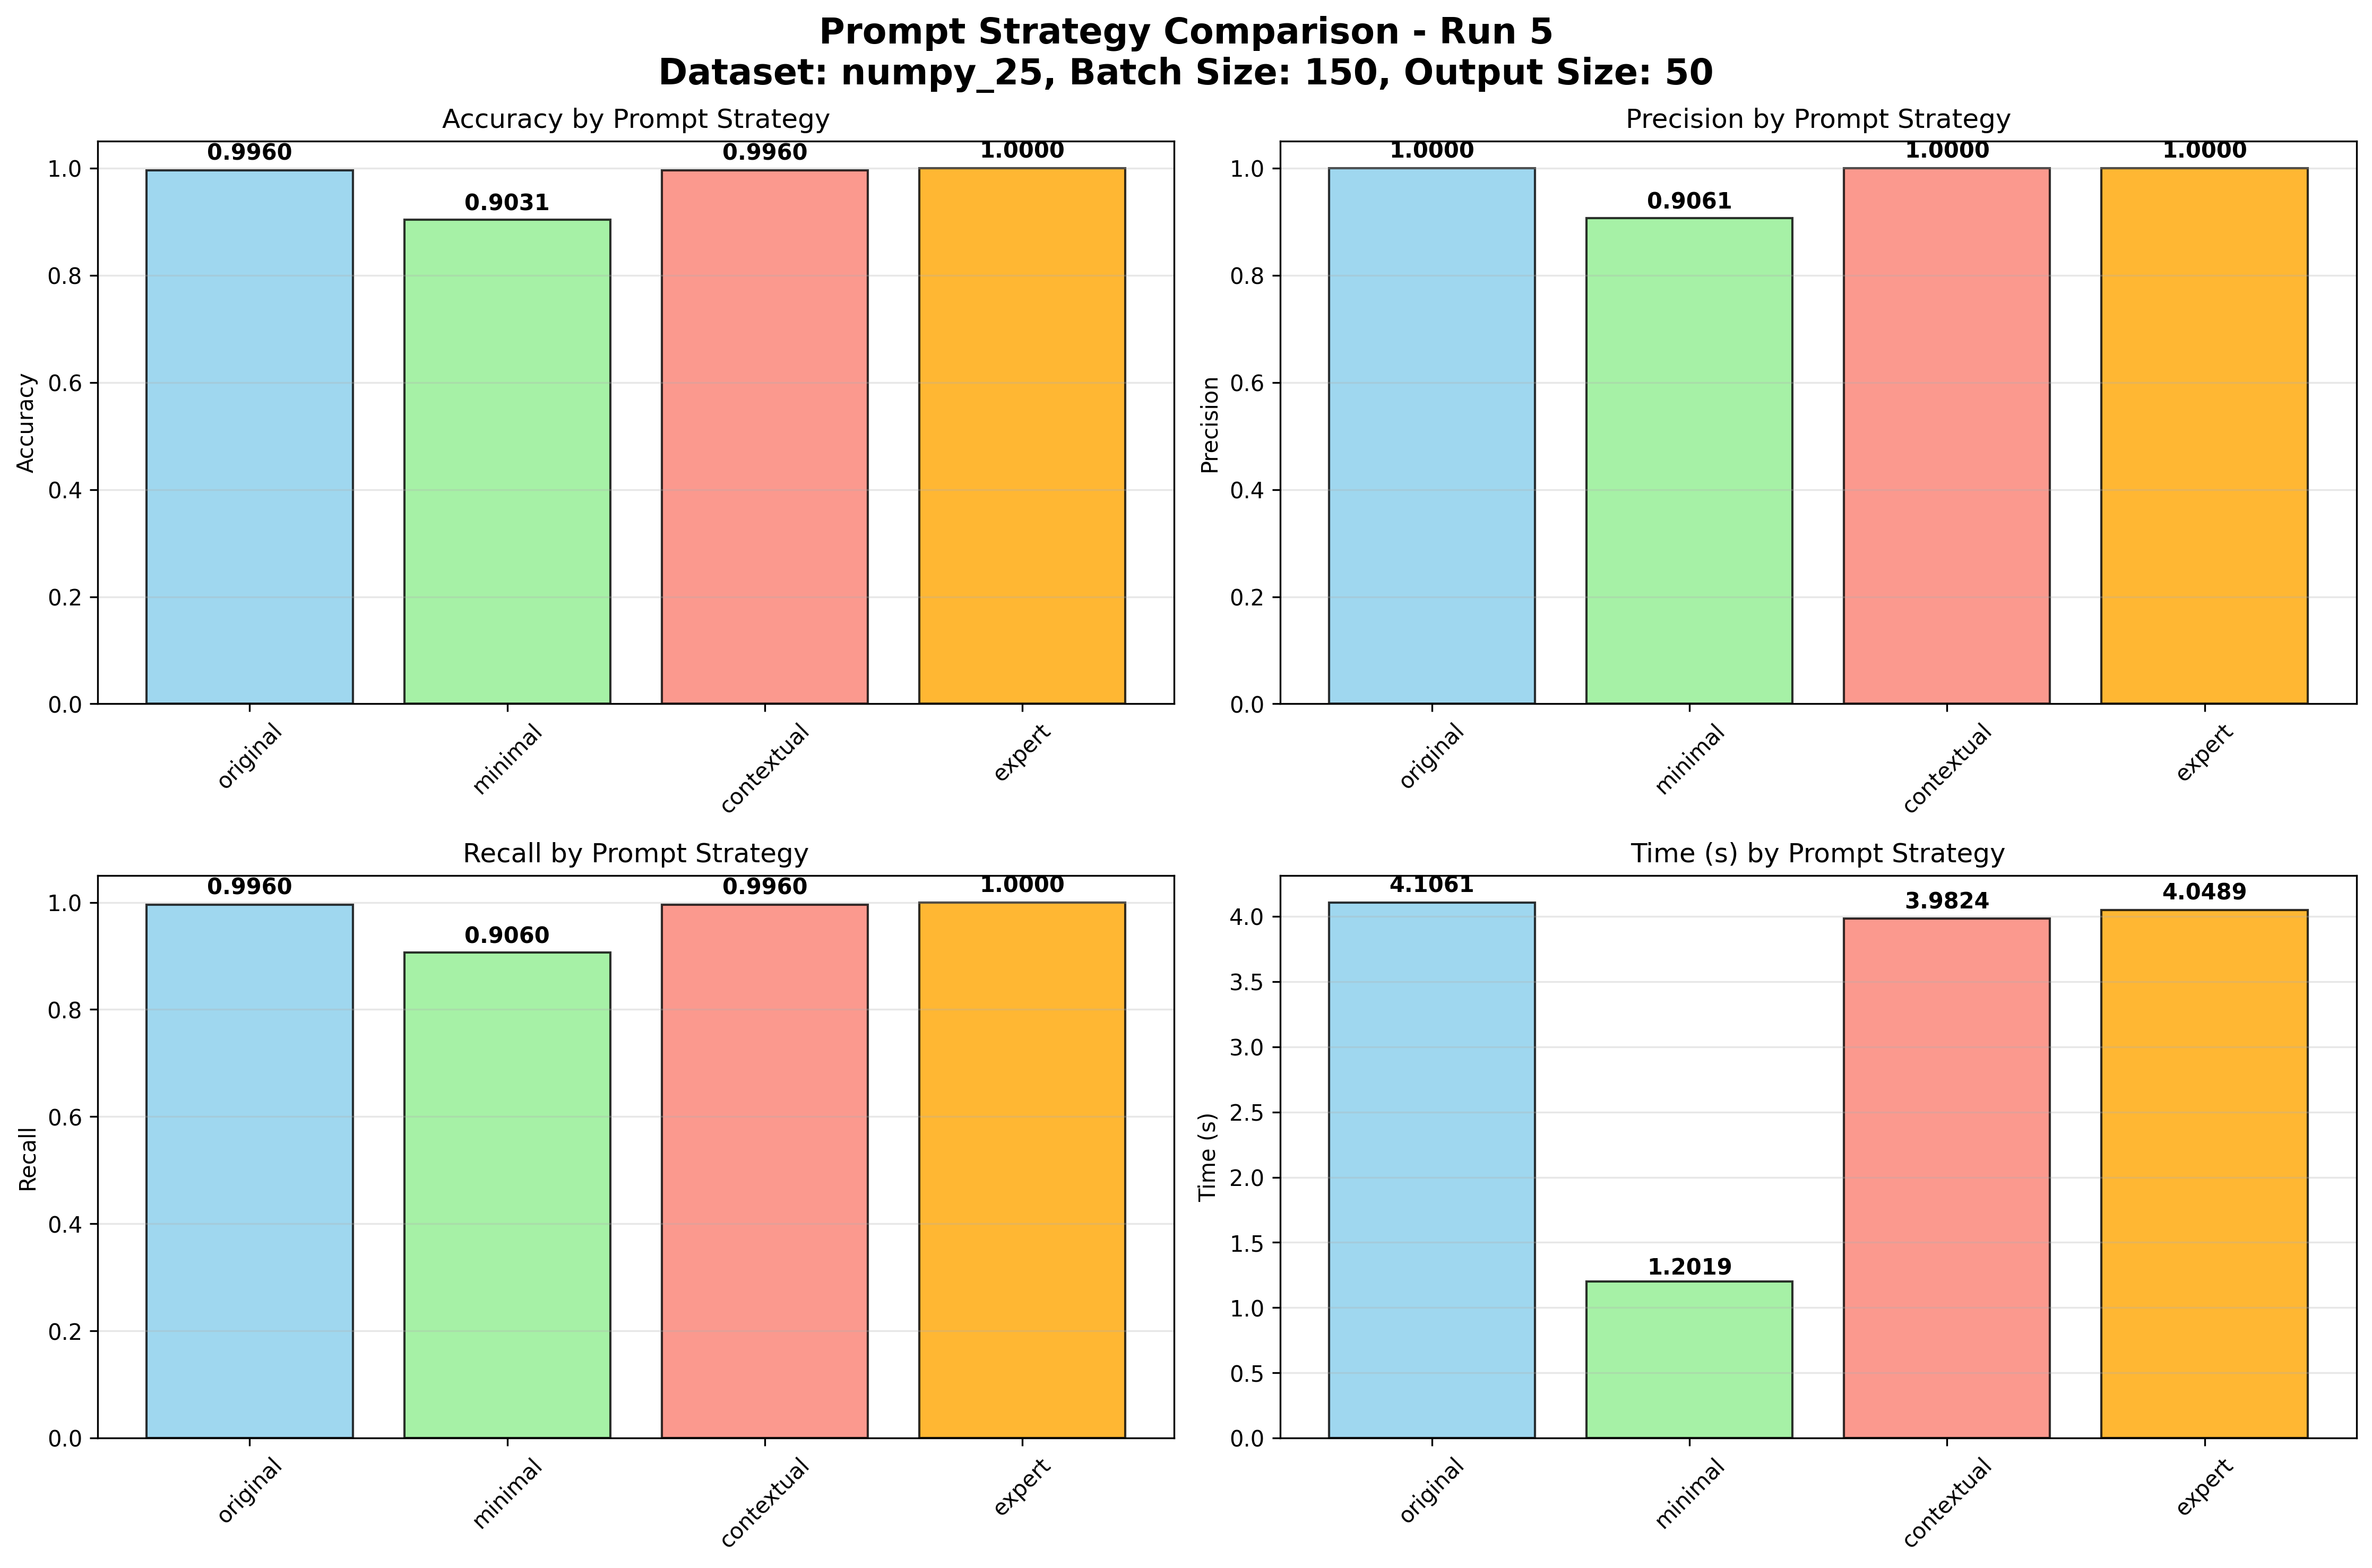
\includegraphics[width=\columnwidth]{prompt_comparison_run5.png}
% \caption{Performance comparison across different prompt configurations showing accuracy metrics and inference times.}
% \label{fig:prompt-comparison}
% \end{figure*}

Table 3 compares the prompt strategies, and reveals slight performance differences between the original, contextual, and expert prompt settings across all four metrics, notably, the minimal prompt has a higher accuracy by 6-12\%, while also requiring less than half the time than all of the other prompt strategies. 

This finding suggests that reducing prompt complexity allows the model to focus primarily on pattern detection without being distracted by extensive contextual information or domain-specific instructions. The simplified approach produces significant improvements in processing speed, indicating that overly complex prompts may introduce unnecessary cognitive overhead for the language model, and that the context provided is likely redundant and does not benefit in these small batch cases. These findings are consistent with other datasets as well. 

\begin{table}[!htbp]
\centering
\caption{Prompt Strategy Comparison (lrange\_50)}
\small
\label{tab:prompt-strategy-comparison}
\begin{tabular}{@{}lrrrr@{}}
\toprule
\textbf{Prompt} & \textbf{Accuracy (\%)} & \textbf{Precision (\%)} & \textbf{Recall (\%)} & \textbf{Time (s)} \\
\midrule
Original & 49.7 & 63.1 & 66.5 & 4.71 \\
Minimal & 56.2 & 68.0 & 71.7 & 1.82 \\
Contextual & 44.5 & 60.4 & 59.0 & 4.72 \\
Expert & 51.6 & 64.9 & 67.5 & 4.62 \\
\bottomrule
\end{tabular}
\end{table}


\subsection{Dataset Performance Analysis}

Our evaluation across multiple program traces reveals that Gemini's performance varies dramatically depending on the specific workload characteristics. While the model performs well on many traces, it shows poor results on others, highlighting the importance of program behavior patterns for LLM-based prefetching.

\begin{table}[!htbp]
\centering
\caption{Dataset Average Performance Summary}
\label{tab:dataset-summary}
\small
\begin{tabular}{@{}lcccc@{}}
\toprule
\textbf{Dataset} & \textbf{Accuracy (\%)} & \textbf{Precision (\%)} & \textbf{Recall (\%)} & \textbf{Time (s)}\\
\midrule
cactu\_25 & 78.7 & 83.8 & 83.2 & 3.57 \\
cactu\_50 & 95.3 & 97.2 & 97.2 & 4.01 \\
\midrule
lrange\_25 & 41.6 & 59.1 & 57.8 & 4.14 \\
lrange\_50 & 46.3 & 61.4 & 62.4 & 4.16 \\
\midrule
mcf\_25 & 0.4 & 0.9 & 0.8 & 5.01 \\
mcf\_50 & 97.4 & 100.0 & 97.4 & 3.55 \\
\midrule
numpy\_25 & 89.4 & 100.0 & 89.4 & 4.00 \\
numpy\_50 & 99.4 & 100.0 & 99.4 & 3.81 \\
\midrule
omnetpp\_25 & 20.6 & 37.9 & 27.8 & 4.19 \\
omnetpp\_50 & 11.3 & 19.7 & 19.2 & 3.87 \\
\midrule
pr\_25 & 98.0 & 90.0 & 98.0 & 3.51 \\
pr\_50 & 100.0 & 100.0 & 100.0 & 3.64 \\
\midrule
ycsb\_25 & 2.7 & 4.7 & 4.6 & 5.33 \\
ycsb\_50 & 1.6 & 3.1 & 3.0 & 5.34 \\
\bottomrule
\end{tabular}
\end{table}

Comparing cache sizes, programs generally show similar performance between 25-line and 50-line context windows, with one notable exception: the MCF trace. For MCF, the 25-line configuration achieves less than 0.5\% accuracy, while the 50-line version reaches 97.4\% accuracy.

This performance variability suggests that certain program types are well-suited for LLM-based prefetching, likely those with sequential patterns that fit within 100-200 line scopes and can be effectively captured in one-shot prompts. Conversely, programs with irregular or highly complex memory access patterns may not benefit from this approach. The cache size analysis further demonstrates that the granularity of context provided to the model significantly influences the quality of generated predictions, with some programs requiring larger context windows to reveal their underlying patterns.

\subsection{Prediction Path Visualization}

\begin{figure}[H]
  \includegraphics[width=\linewidth]{pred.png}
  \caption{Prediction and Ground Truth}
  \label{fig:predPath}
\end{figure}

The prediction path visualization demonstrates the model's ability to align with and self-correct against ground truth patterns, even under complex and highly varying execution conditions. This adaptive behavior suggests that LLMs can capture nuanced program behaviors that might challenge traditional prefetching algorithms, though this capability is highly dependent on the specific program characteristics and context provided.


% \subsection{Overall Performance Comparison}
% Figure~\ref{fig:performance-overview} presents the overall performance comparison across all test configurations, showing hit rate, precision, recall, and accuracy metrics.








% \begin{figure}[t]
% \centering
% \begin{tikzpicture}
% \begin{axis}[
%     width=\columnwidth,
%     height=5cm,
%     xlabel={Metric},
%     ylabel={Performance (\%)},
%     ymin=60, ymax=85,
%     legend pos=north east,
%     symbolic x coords={Hit Rate,Precision,Recall,Accuracy},
%     xtick=data,
%     x tick label style={anchor=east},
% ]

% \addplot[color=blue,mark=square,thick] coordinates {
%     (Hit Rate,72.3) (Precision,69.1) (Recall,74.5) (Accuracy,67.8)
% };

% \addplot[color=red,mark=triangle,thick] coordinates {
%     (Hit Rate,76.1) (Precision,73.8) (Recall,78.4) (Accuracy,71.2)
% };

% \legend{Gemini 2.0,Gemini 2.5}
% \end{axis}
% \end{tikzpicture}
% \caption{Performance Comparison: Gemini 2.0 vs 2.5}
% \label{fig:model-comparison}
% \end{figure}

\subsection{Hyperparameter Sweep Results}

\begin{figure}
    \centering
    \includegraphics[width=1\linewidth]{accuracysweep.png}
    \caption{Caption}
    \label{fig:placeholder}
\end{figure}

\begin{figure}
    \centering
    \includegraphics[width=1.\linewidth]{timesweep.png}
    \caption{Caption}
    \label{fig:placeholder}
\end{figure}
Figures 4 and 5 show the accuracy heatmap plotting batch and output size, where lighter colors indicate better model performance. Performance degrades significantly at batch size 200, which suggests a soft batch size ceiling beyond which the transformer struggles to maintain relationships within the data, likely due to memory limitations or attention constraints.
Optimal performance occurs at moderate output sizes of 30-40 addresses, with the three best-performing configurations being (100,40), (125,30), and (175,30), achieving accuracies of 1.000, 1.000, and 0.987 respectively. Batch sizes below 200 demonstrate consistently strong performance, indicating robust scalability within this range.
The timing analysis reveals that completion time is governed by output size rather than batch size. Average completion times increase approximately linearly with output size (from ~1.4s at size 10 to ~5.9s at size 70), while showing minimal variation across different batch sizes for equivalent output sizes. This pattern suggests that the bottleneck lies in the generation process rather than input processing, where each additional output token requires similar processing time regardless of batch size, consistent with autoregressive transformer behavior during inference. \cite{sheebaelhamd2025quantization}

% \begin{table}[h]
% \centering
% \caption{Context Window Size Impact Analysis}
% \label{tab:context-analysis}
% \begin{tabular}{@{}lrrrr@{}}
% \toprule
% Input Size & Hit Rate & Precision & Recall & Inference Time \\
% \midrule
% 50 & 72.3\% & 69.1\% & 74.5\% & 847ms \\
% 64 & 75.8\% & 72.4\% & 78.1\% & 1023ms \\
% 100 & 78.2\% & 75.6\% & 81.3\% & 1489ms \\
% 128 & 78.9\% & 75.2\% & 81.3\% & 1647ms \\
% 200 & 79.1\% & 75.8\% & 82.1\% & 2156ms \\
% \bottomrule
% \end{tabular}
% \end{table}

% \begin{figure}[t]
% \centering
% \begin{tikzpicture}
% \begin{axis}[
%     width=\columnwidth,
%     height=5cm,
%     xlabel={Training → Evaluation Dataset},
%     ylabel={Hit Rate (\%)},
%     ymin=60, ymax=85,
%     symbolic x coords={25→25,25f→25,50→25,50f→25,25f→25f,50f→50},
%     xtick=data,
%     x tick label style={rotate=30,anchor=east},
%     nodes near coords,
%     nodes near coords align={vertical},
% ]

% \addplot[color=blue,mark=square,thick] coordinates {
%     (25→25,72.3) (25f→25,68.5) (50→25,71.2) (50f→25,74.8) (25f→25f,82.4) (50f→50,77.6)
% };

% \end{axis}
% \end{tikzpicture}
% \caption{Cross-Dataset Generalization Performance}
% \label{fig:cross-dataset}
% \end{figure}

% \subsection{Limitations and Challenges}

% \textbf{Fine tuning}: While fine tuning was intended to be an important portion to this project, the tuning process was too costly (about $\$30$ per trained model) and the results performed poorer than the one-shot prompts, suggesting that some part of the methodology is not properly implemented. 

% \textbf{Inference Latency:} Current inference times (650-2000ms) are too high for real-time prefetching applications. Significant optimization would be required for practical deployment.

% \textbf{Response Reliability:} Success rates vary from 89-99\%, with larger context windows and complex prompts showing higher failure rates. Robust error handling is essential for production systems.

% \textbf{Pattern Complexity:} While LLMs excel at learning complex patterns, they occasionally fail on simple sequential patterns that traditional prefetchers handle trivially.

% \subsection{Practical Implications}

% Despite current limitations, our results suggest several promising directions:

% \textbf{Hybrid Approaches:} Combining LLM-based prefetching with traditional hardware prefetchers could leverage the strengths of both approaches.

% \textbf{Offline Training:} Pre-training specialized models on program-specific traces could improve accuracy while reducing inference requirements.

% \textbf{Hierarchical Prediction:} Using LLMs for high-level pattern prediction and traditional methods for fine-grained prefetching could balance accuracy and performance.

% \section{Future Work}
% \label{sec:future}

% Several research directions emerge from our work:

% \subsection{Model Optimization}
% \begin{itemize}
% \item Fine-tuning Gemini models specifically for memory access prediction
% \item Exploring smaller, specialized models for reduced inference latency
% \item Investigating quantization and pruning techniques for deployment efficiency
% \end{itemize}

% \subsection{System Integration}
% \begin{itemize}
% \item Developing hardware-software interfaces for LLM-enhanced prefetching
% \item Designing adaptive systems that switch between LLM and traditional prefetching
% \item Exploring edge deployment scenarios with local model inference
% \end{itemize}

% \subsection{Advanced Techniques}
% \begin{itemize}
% \item Multi-modal approaches combining code analysis with execution traces
% \item Reinforcement learning for dynamic prefetching policy adaptation
% \item Federated learning for cross-application pattern sharing
% \end{itemize}

% \subsection{Broader Applications}
% \begin{itemize}
% \item Extending to other system optimization problems (branch prediction, cache replacement)
% \item Investigating domain-specific applications (database query optimization, network traffic prediction)
% \item Exploring real-time system requirements and constraints
% \end{itemize}

% \section{Conclusion}
% \label{sec:conclusion}

% This paper presents the first comprehensive evaluation of large language models for memory prefetching, specifically examining Google's Gemini model across multiple configurations and datasets. Our systematic experimental methodology, encompassing 10 distinct test configurations, provides valuable insights into the potential and limitations of LLM-enhanced prefetching.

% \textbf{Key Contributions:} We demonstrate that Gemini can achieve hit rates of up to 84.2\% on memory access prediction tasks, significantly outperforming many traditional prefetching approaches on complex, irregular access patterns. Our analysis reveals that model version, context window size, and prompt engineering strategies all significantly impact performance.

% \textbf{Practical Impact:} While current inference latencies limit immediate deployment, our results suggest that LLM-based prefetching could be viable for offline analysis, hybrid prefetching systems, or specialized hardware implementations. The ability to learn complex, application-specific patterns represents a significant advancement over traditional approaches.

% \textbf{Research Directions:} Future work should focus on model optimization for reduced inference latency, system-level integration challenges, and exploration of hybrid approaches that combine the strengths of LLM and traditional prefetching methods.

% Our work establishes a foundation for the emerging field of AI-enhanced system optimization and demonstrates the potential for large language models to address long-standing challenges in computer architecture and systems design.

% %%
% %% Acknowledgments section
% \begin{acks}
% We thank our colleagues for valuable discussions and feedback throughout this research. We also acknowledge the computational resources provided by our institution's high-performance computing facility and Google's Gemini API access program. 
% \end{acks}

% %%
% Bibliography - make sure to create your references.bib file
% \bibliographystyle{ACM-Reference-Format}
% \bibliography{references.bib}


% \end{document}
\subsection{Limitations and Challenges}

\textbf{Fine tuning}: While fine tuning was intended to be an important portion to this project, the tuning process was too costly (about $\$30$ per trained model) and the results performed poorer than the one-shot prompts, suggesting that some part of the methodology is not properly implemented.

\textbf{Inference Latency:} Current inference times (130ms at the fastest) are too high for real-time prefetching applications when compared to normal . Significant optimization would be required for practical deployment.

\textbf{Parameter-Dependent Reliability:} Response reliability is highly sensitive to configuration parameters, with success rates varying dramatically from 0.05-100\% depending on context window size, prompt complexity, and dataset characteristics. This parameter sensitivity makes robust deployment challenging and requires extensive tuning for each application scenario.

\textbf{Economic Feasibility:} After processing approximately 2000 batches, API costs reached \$0.50, which may seem modest but becomes prohibitive when scaled to continuous prefetching requirements. For production systems requiring millions of predictions daily, current pricing models make LLM-based prefetching economically unfeasible.

% \textbf{Hybrid System Complexity:} While combining LLM-based prefetching with traditional hardware prefetchers could leverage the strengths of both approaches, such hybrid systems introduce significant complexity in coordination, fallback mechanisms, and dynamic switching between prediction methods, potentially offsetting the benefits.

\section{Future Work}
\label{sec:future}


\subsection{Model Optimization and Fine-tuning}
Investigating fine-tuning approaches designed for memory access prediction could potentially improve both speed and accuracy. Future work should explore whether domain-specific training can reduce the model size requirements while maintaining prediction quality, addressing both latency and cost concerns.

\subsection{Advanced Prompt Engineering}
Our results demonstrate that prompt strategy significantly impacts both performance and inference time. Future research should systematically explore more sophisticated prompt engineering techniques, including few-shot learning approaches, chain-of-thought prompting, and adaptive prompt selection based on program characteristics. The minimal prompt performed best in these small batch scenarios, but this conclusion is not generalizable to every scenario.

\subsection{Model Diversity and Scaling}
Comprehensive evaluation across different Gemini versions and alternative LLMs (Claude, GPT-4, specialized smaller models) could reveal optimal model architectures for prefetching tasks. Additionally, investigating how input-output dimensions scale with different model capabilities could improve deployment strategies.


\section{Conclusion}
\label{sec:conclusion}

This paper presents an evaluation of large language models for memory prefetching, demonstrating both the remarkable potential and significant limitations of applying LLMs to low-level system optimization tasks. There is certainly more work to be done in this area, and it is likely that machine learning integrates into mainstream prefetching systems in the near future.

\textbf{Performance Potential:} Our results reveal that under optimal conditions, Gemini can achieve perfect prediction accuracy, correctly predicting 40/40 memory addresses in a single batch. However, this performance is highly variable, with some configurations yielding less than 0.5\% accuracy, highlighting the sensitivity of LLM-based approaches to both dataset characteristics and configuration parameters.

\textbf{Practical Assessment:} While LLMs show promise for memory prefetching, our analysis suggests that current large language models are likely too heavyweight for practical deployment in real-time prefetching systems. The combination of high inference latency, substantial computational costs, and parameter sensitivity creates significant barriers to production adoption.

\textbf{Alternative Value Proposition:} Despite deployment challenges, LLMs could serve a valuable role in prefetching research and development. Their ability to identify complex, non-obvious patterns in memory access traces could be useful in the design of more efficient traditional prefetchers. By using LLMs as pattern discovery tools rather than production prefetchers, researchers could leverage their pattern recognition capabilities to develop insights that guide the creation of more specialized prefetching algorithms.

% \textbf{Research Impact:} Our work establishes important baseline performance metrics and identifies key challenges for AI-enhanced system optimization. The dramatic variability in prediction accuracy—from near-perfect to nearly useless—underscores the need for robust evaluation methodologies and highlights the complexity of applying general-purpose AI models to specialized system tasks.


\begin{acks}
I thank Systopia for providing the datasets that made this research possible. I am grateful to Shaurya Patel and Sasha Federova for providing the opportunity to work on this project and for their guidance throughout the research process. I also acknowledge the computational resources provided by institution's high-performance computing facility and Google's Gemini API.
\end{acks}

%%
%% Bibliography - make sure to create your references.bib file
\bibliographystyle{ACM-Reference-Format}
\bibliography{references.bib}

\end{document}